\section{Reconhecimento Facial}

O reconhecimento facial é uma das atividades mais comuns realizadas diariamente por seres vivos dotados de certa inteligência. Essa simples atividade vem despertando o interesse de pesquisadores que trabalham com Visão Computacional e Inteligência Artificial. O objetivo desses pesquisadores é de construir sistemas artificiais capazes de realizar o reconhecimento de faces humanas e a partir desta capacidade construir os mais diferentes tipos de aplicações: sistemas de vigilância, controles de acesso, definções automáticas de perfis, entre outros \cite{oliveira}.

No anos 70, os estudos do reconhecimento facial eram baseados sobre atributos faciais mensuráveis como olhos, nariz, sobrancelhas, bocas, entre outros. Porém, os recursos computacionais eram escassos e os algoritmos de extração de características eram ineficiêntes. Nos anos 90, as pesquisas na área ressurgiram, inovando os métodos existentes \cite{hong, saocarlos} e disseminando a técnica.

Um dos motivos que incentivou os diversos estudos sobre reconhecimento facial são as vantagens que o mesmo possui em relação a impressão digital e a íris.  No reconhecimento por impressão digital, a desvantagem consiste no fato que nem todas as pessoas possuem uma impressão digital com ``qualidade'' suficiente para ser reconhecida por um sistema. Já o reconhecimento por íris apresenta uma alta confiabilidade e larga variação, sendo estável pela vida toda. Porém, a desvantagem está relacionada ao modo de captura da íris que necessita de uma alinhamento entre a câmera e os olhos da pessoa \cite{saocarlos}. 

Basicamente existem duas particularidades que fazem da face uma característica biométrica bastante atrativa \cite{drovetto}:

	\begin{enumerate}
		\item A aquisição da face é feita de forma fácil e não-intrusiva;
		\item Possui uma baixa privacidade de informação: como a face é exposta constantemente, caso uma base de faces seja roubada, essas informações não representam algum risco e não possibilitam um uso impróprio;
	\end{enumerate}

Umas das maiores dificuldades dos sistemas de reconhecimento é tratar a complexidade dos padrões visuais. Mesmo sabendo que todas as faces possuem padrões reconhecidos, como boca, olhos e nariz, elas também possuem variações únicas que devem ser utilizadas para determinar as características relevantes. Outra dificuldade encontrada em relação a essas características é que elas possuem uma larga variação estatística para serem consideradas únicas para cada indivíduo. O ideal seria que a variância inter-classe seja grande e a intra-classe pequena, pois assim imagens de diferentes faces geram os códigos mais diferentes possíveis, enquanto imagens de uma mesma face geram os códigos mais similares possíveis. Portanto, estabelecer uma representação que capture as características ideias é um difícil problema \cite{saocarlos}.

Do ponto de vista geral, o recohecimento facial continua sendo um problema aberto por causa de várias dificuldades que aumentam a variância intra-classe \cite{hong}. Entre estas, destacamos as mais comuns \cite{saocarlos}:

	\begin{itemize}
		\item iluminação;
		\item ângulos e poses;
		\item expressões;
		\item comésticos e acessórios;
		\item extração da face do contexto ou do fundo;
	\end{itemize}

No contexto de identificação, o reconhecimento facial se resume no reconhecimento de um ``retrato'' frontal, estático e controlado. Estático pois os ``retratos'' utilizados nada mais são que imagens, podendo ser tanto de intensidade quanto de profunidade e controlado pois a iluminação, o fundo, a resolução dos dispositivos de aquisição e a distância entre eles e as faces são essencialmente fixos durante o processo de aquisição da imagem \cite{hong}.

Basicamente, o processo de reconhecimento facial pode ser divido em duas tarefas principais \cite{hong}:

	\begin{enumerate}
		\item Detecção de faces em imagens;
		\item Reconhecimento das faces encontradas;
	\end{enumerate}

Falaremos dessas duas tarefas separadamente nas próximas subseções.

% ################################################################################################################################################

\subsection{Detecção de Faces em imagens}
	
A primeira etapa para o reconhecimento de faces é a detecção de um rosto, e a partir daí a comparação do mesmo com modelos conhecidos pelo sistema \cite{hong, oliveira}. Em um sistema de reconhecimento facial, tanto o tempo de resposta quanto a confiabilidade desta etapa influência diretamente no desempenho e o emprego deste sistema \cite{oliveira}.

A detecção de faces é definida como o processo que determina a existência ou não de faces em uma imagem e uma vez encotrada alguma face, sua localização deve ser apontada através de um enquadramento ou através de suas coordenadas dentro da imagem \cite{oliveira}. A Figura \ref{enquadramentoRosto} representa um exemplo da detecção de uma face em uma imagem.

	\begin{figure}[hbt]
		\begin{center}
			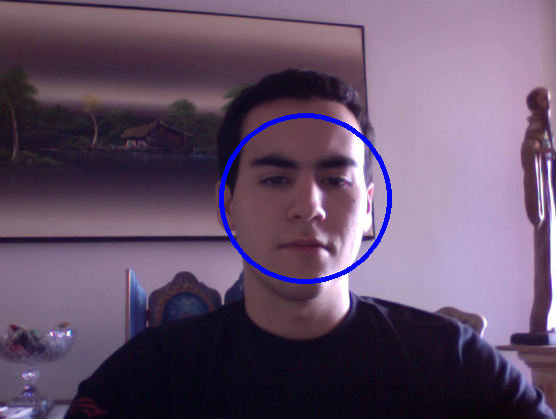
\includegraphics[height=9.5cm,width=12.5cm]{figuras/2.FundamentacaoTeorica/enquadramentoRosto.png}
		\end{center}
		\caption{Exemplo de um processo de detecção de uma face em uma imagem.}
		\label{enquadramentoRosto}
	\end{figure}

O processo de detecção de faces geralmente é dificultado pelas seguintes razões mostradas a seguir:

	\begin{enumerate}
		\item \textbf{Pose}: as imagens de uma face podem variar de acordo com a posição relativa entre a camêra e a face (frontal, 45 graus, perfil, ``de cabeça para baixo''), e com isso algumas características da face, como olhos e nariz, podem ficar parcialmente ou totalmente ocultadas \cite{yang}.
		\item \textbf{Presença de acessórios}: características faciais básicas importantes para o processo de detecção podem ficar ocultadas pela presença de acessórios, como óculos, bigode, barba, entre outros \cite{oliveira, yang}. 
		\item \textbf{Expressões faciais}: embora a maioria das faces apresente estruturas semelhantes (olhos, bocas, nariz, entre outros) e são dispostas aproximadamente na mesma configuração de espaço, pode haver um grande número de componentes não rigídos e texturas diferentes entre as faces. Um exemplo são as flexibilizações causadas pelas expressões faciais \cite{oliveira, yang};
		\item \textbf{Obstrução}: faces podem ser obstruídas por outros objetos. Em uma imagem com várias faces, uma face pode obstruir outra \cite{yang}.
		\item \textbf{Condiçoes da imagem}: a não previsibilidade das condições da imagem em ambientes sem restrições de ilimuniação, cores e objetos de fundo \cite{oliveira, yang}.
	\end{enumerate}

Atualmente, já existem diferentes métodos/técnicas de detecção de faces. Faleremos um pouco sobre os métodos baseados em imagens de itensidade e de cor e depois falaremos sobre os baseados em imagens 3D.

% Os métodos baseados em imagens de intensidade e cor podem ser divididos em 4 categorias \cite{yang}:

% 	\begin{enumerate}
% 		\item \textbf{``Knowladge-based methods'':} métodos, desenvolvidos principalmente para localização facial, beaseados em regras derivadas do conhecimento dos pesquisadores do que constitui uma típica face humana. Normalmente, captura as relações existentes entre as características faciais. É fácil econtrar regras que descrevem as caracterísicas faciais. Por exemplo, uma face sempre é constituída por dois olhos simétricos, um nariz e uma boca. As relações entre essas características podem ser representadas pelas distâncias relativas e posições.  \cite{yang};

% 		\item \textbf{``Feature invariant approaches'':} esses algoritmos tem como objetivo principal encontrar as características estruturais que existem mesmo quando a postura, ``ponto de vista'', condições de iluminação variam. E por meio dessas características localizar a face. São desenvolvidos principalmente para localização facial \cite{yang};

% 		\item \textbf{``Template matching methods'':} vários padrões comuns de um rosto são armazenados tanto para descrever o rosto como um todo quanto para descrever as características faciais separadamente. As correlações entre as imagens de entrada e os padrões armazenados são comuptados para detecção. Esses métodos são desenvolvidos para serem utlizados como localização e detecção facial \cite{yang};

% 		\item \textbf{``Appearence-based methods'':} Em contraste com os métodos do item anterior, os modelos são retirados de um conjunto de imagens de treinamento que devem capturar a variabilidade da face. Esses modelos retirados são utilizados para detecção. São métodos desenvolvidos principalmente para detecção de faces \cite{yang};

% 	\end{enumerate}

Um problema relacionado e muito importante é como avaliar a performance dos métodos de detecção de faces propostos. Com isso, muitas métricas foram adotadas como tempo de aprendizagem, número de amostras necessárias no treinamento e a proporção entre taxas de detecção e ``falso alarme''. Esta última é dificultada pelas diferentes definições para as taxas de detecção e falso alarme adotadas pelos pesquisadores \cite{yang}.




































% ################################################################################################################################################

\subsection{Reconhecimento das Faces encontradas}









